\chapter{Metalware}

This chapter covers the mechanical part of the build.
Note that the construction requires access to a workshop as most parts are custom.

Software:

\begin{itemize}
	\item Autodesk Inventor Professional 2013
\end{itemize}

\section{Frame}

A frame consisting of 2020 aluminium extrusions serves as mechanical backbone for everything.
Other parts, like the base-plate, are connected to it.
In the final steps of the assembly, the frame is lowered into the case with all components attached and fastened to the case.

Navigate to the corresponding section in \cref{bom}.

Assembling the frame is straight forward.
Just watch out to insert the correct nuts into the correct grooves:

\begin{center}
	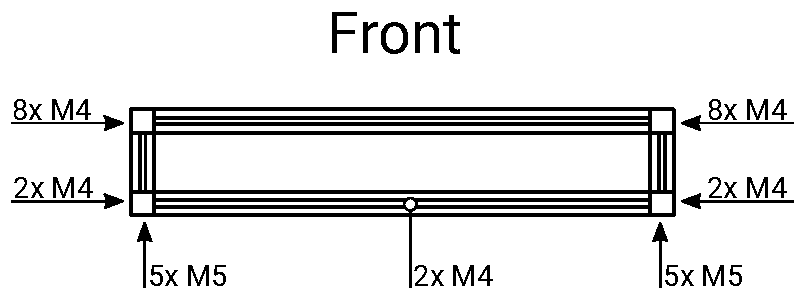
\includegraphics[width=0.95\textwidth]{inc/drawing_frame_front_nuts.pdf}
\end{center}

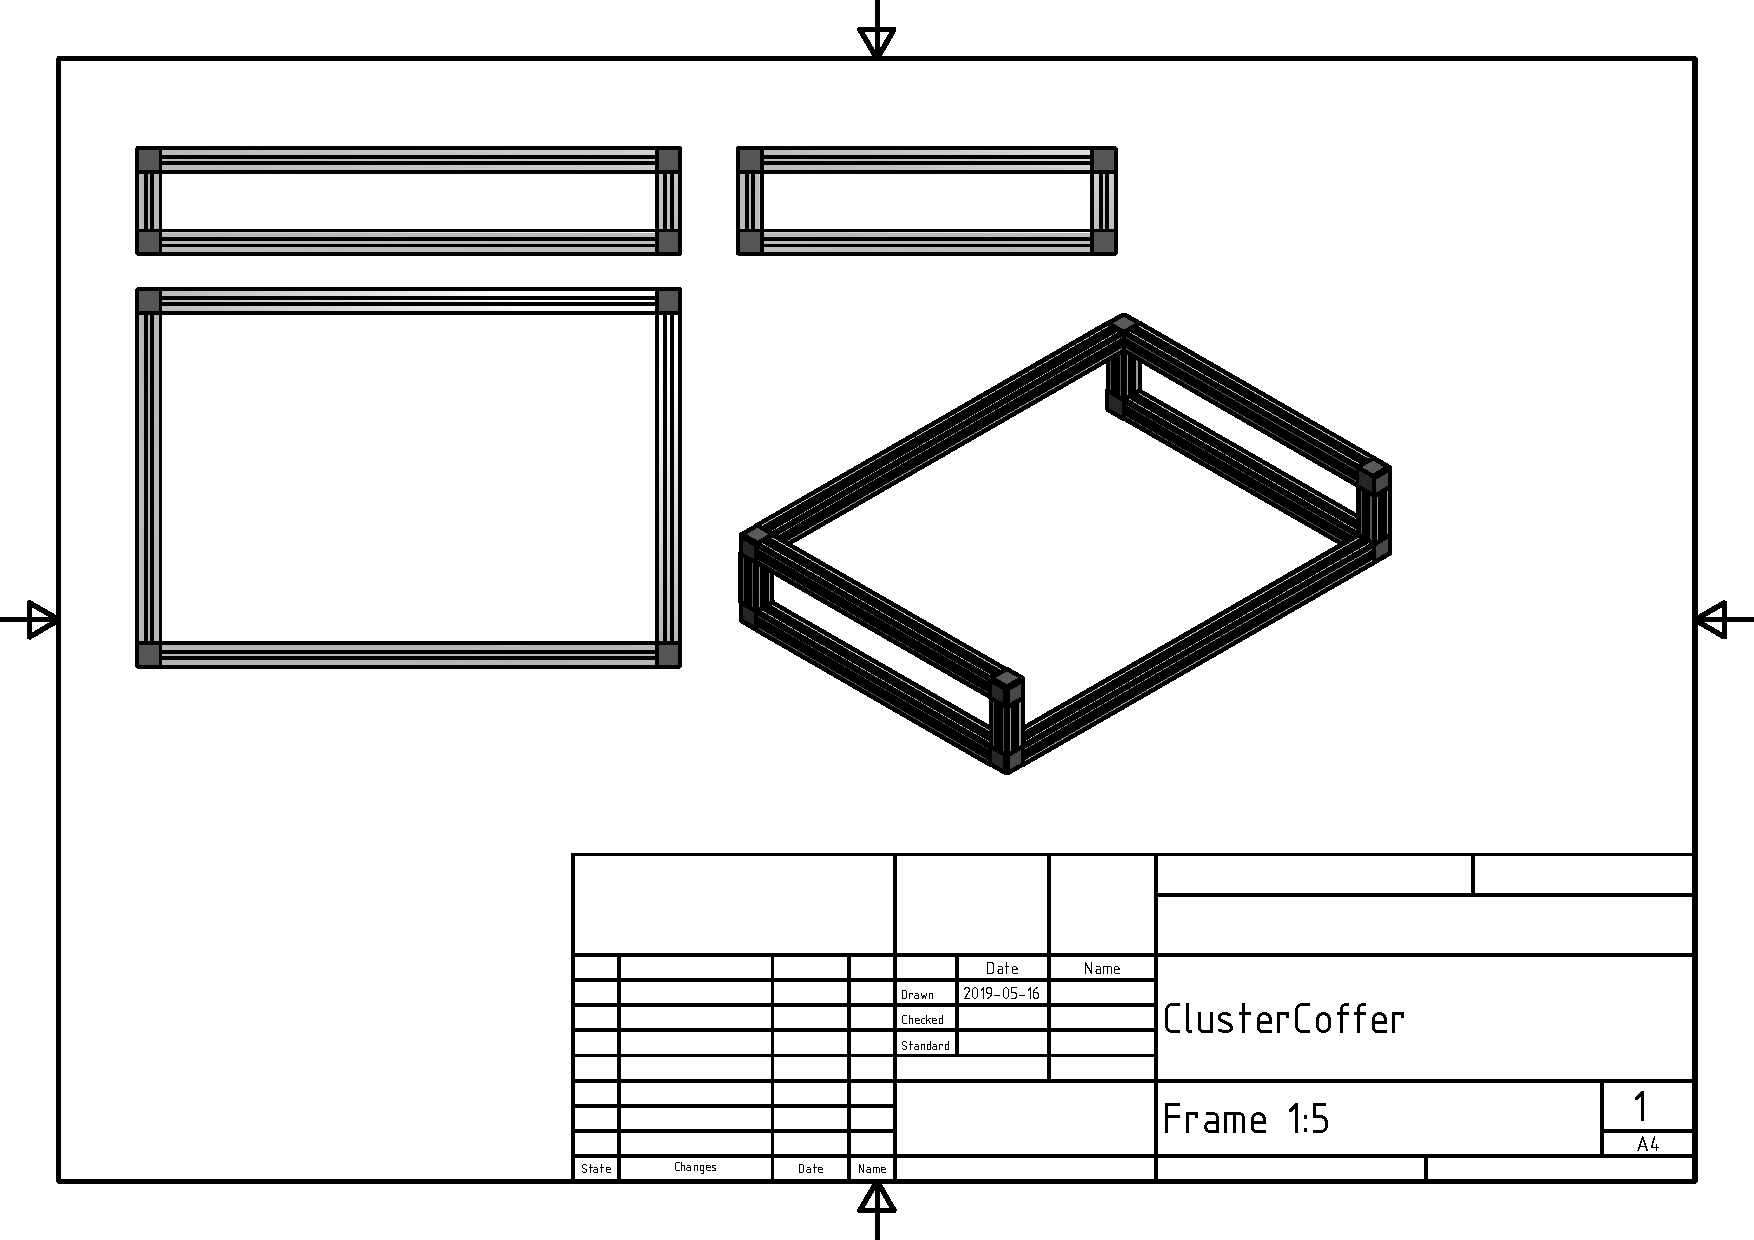
\includepdf[fitpaper]{inc/drawing_frame.pdf}

\section{Base-Plate}

The base-plate is located at the bottom of the assembly.
It holds both power supplies (5 V and 12 V), as well as the switch, and a power conduit box distributing the 230 V mains voltage.

While power supplies and conduit boxes commonly feature mounting holes, the switch requires some gentle modification.
We disassembled the switch and drilled 3 holes into the bottom cover.
This way, it can be mounted to the base-plate using M3 screws.

We also added another hole to the top cover in order to mount a luster terminal.
This comes in handy when wiring up the fans and head node.

The manufacturing drawings at the end of this section are more of a tongue-in-cheek description, but you'll manage.
Holes that belong together are annotated on the same sheet.
The scale is 1:3.

\subsection{Power Supplies}

The beefy 5 V power supply powers the 16 compute nodes.
Head node and fans require 12 V, yet draw considerably less power.

We did not run into any issues with ripple\footnote{\url{https://en.wikipedia.org/wiki/Ripple_(electrical)}}, nevertheless we added capacitors for good measure.
Heat output doesn't seem to be a problem either.

Pay attention to the 230 V terminals of both power supplies.
They should be internal (i.e.\ not accessible from the outside) or at least covered.

\subsection{Switch}

Apart from the 4 new holes, the switch does not feature any other modifications.
The power cord has an angled connector as there is only little clearance between the frame and the mounted switch.
Plug in the power cable before mounting the base-plate to the frame.

\subsection{Mains Power}

Mains power enters the system via a dedicated socket at the back of the case.
This socket also comes with a power switch and a fuse.

On the inside, a cable connects the socket with the conduit box.
The conduit box is connect with the 5 V power supply, the 12 V power supply, and the switch.

Wago-222\footnote{\url{https://www.wago.com/global/installation-terminal-blocks-and-connectors/classic-splicing-connector/p/222-415}} splicing connectors are used.
Large cable ties serve as cable relief.

You can also add additional grounding for the case, frame, or other components if you want.

If any of the components related to 230 V feature open / accessible connectors, consider covering them hot glue.

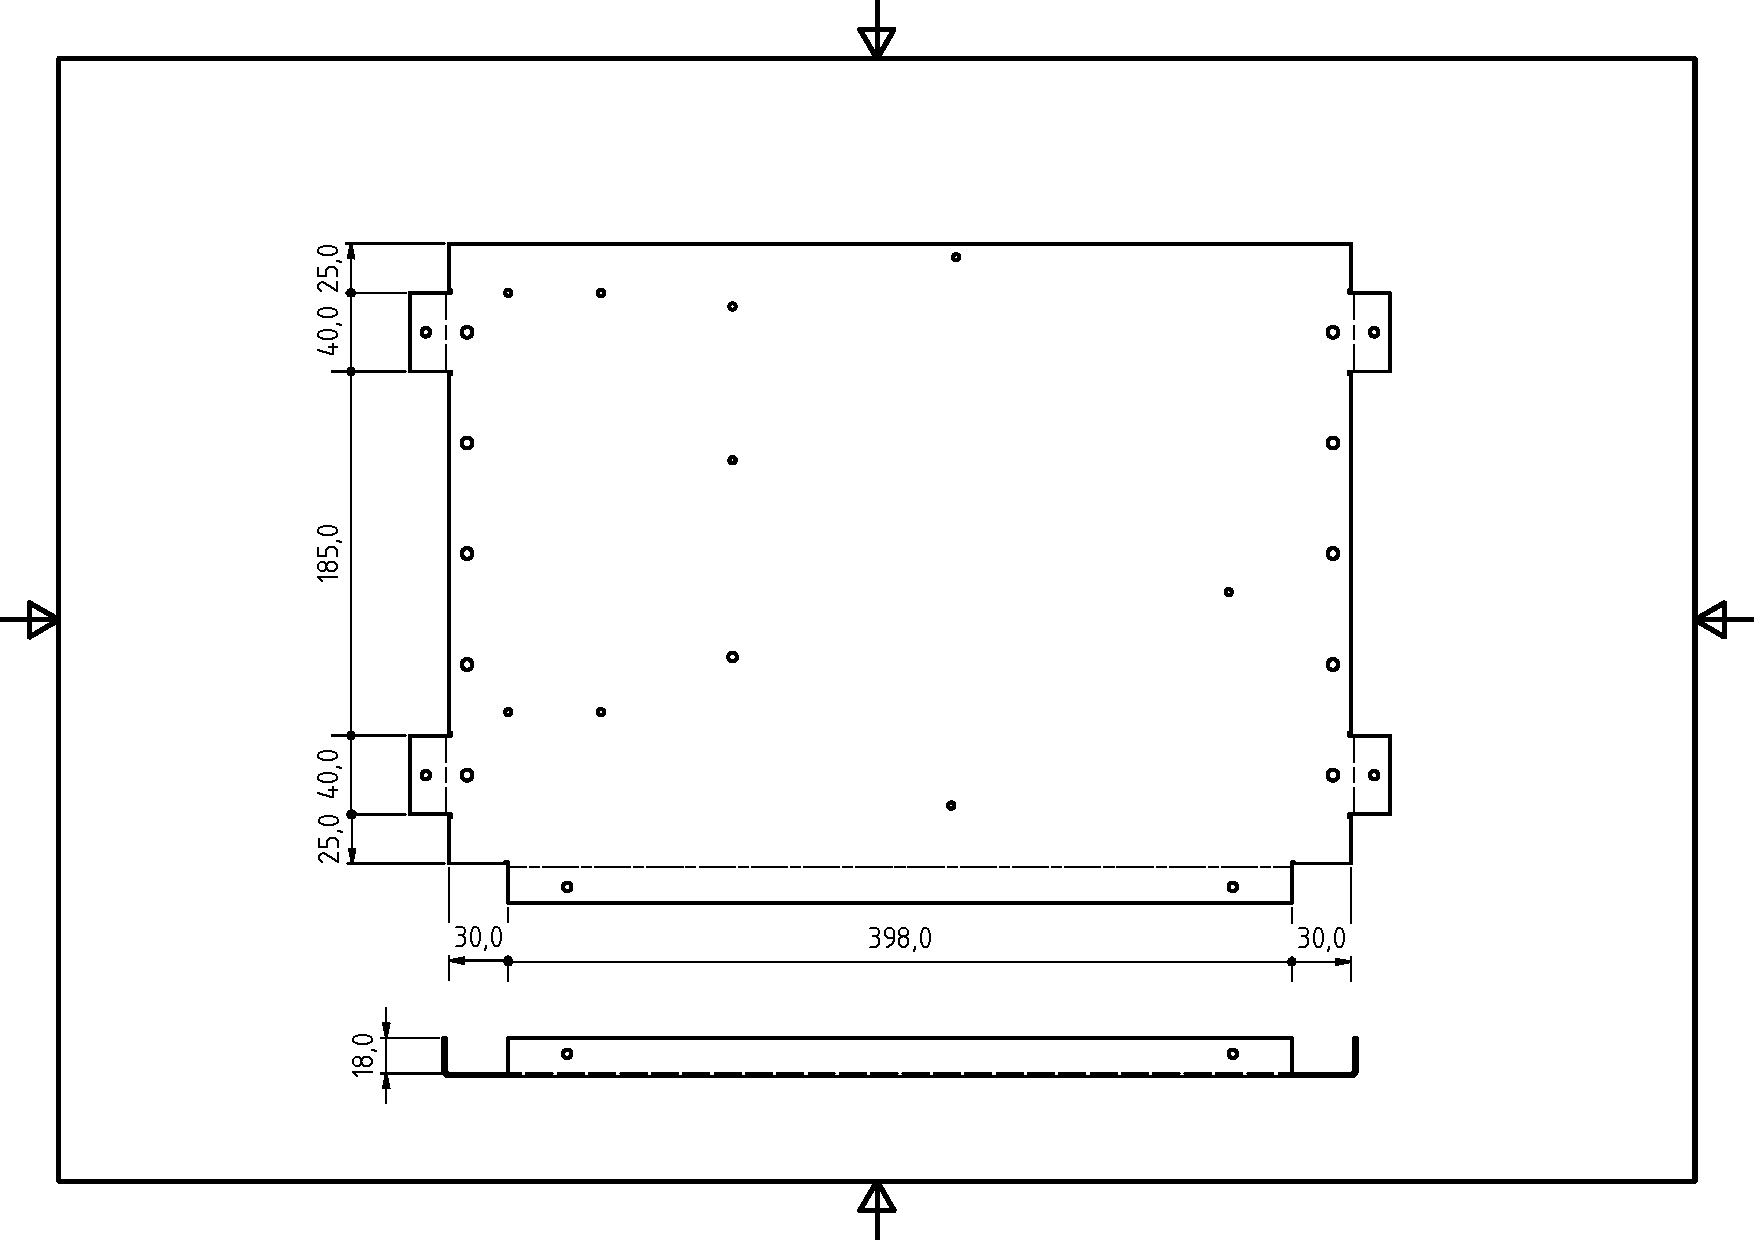
\includepdf[pages=-,fitpaper]{inc/drawing_base_plate.pdf}

\section{V-Mount}

Four V-Mount panels are used to hold all compute nodes.
Each panel holds four compute nodes, four fans, and a power distribution circuit board with switches.

When assembling, start with the fans.
The fans are mounted to the bottom of the panel using countersunk screws.
They push air towards the top, right onto the heatsink.
Ensure the screws sit flush with the surface to prevent any gaps through which air could escape the heatsinks.

The heatsinks of the compute nodes already come with M3 mounting holes that are used for mounting them to the panel.

Consider dealing with the software stuff before mounting them to the panel, as it will be cumbersome to access the micro SD card afterwards.

The power distribution circuit board is added next.
The only mechanical connection is the four toggle switches; however, as there shouldn't be any stress on the board, this should be fine.
Try not to scratch the surface of the panel when tightening the nuts.

After everything has been mounted to the panel, it is recommended to start cable management.
Start by connecting the fan power cables to the power distribution board.
After that, the custom compute node power boards can be attached.

The scale of the following design documents is 1:2.

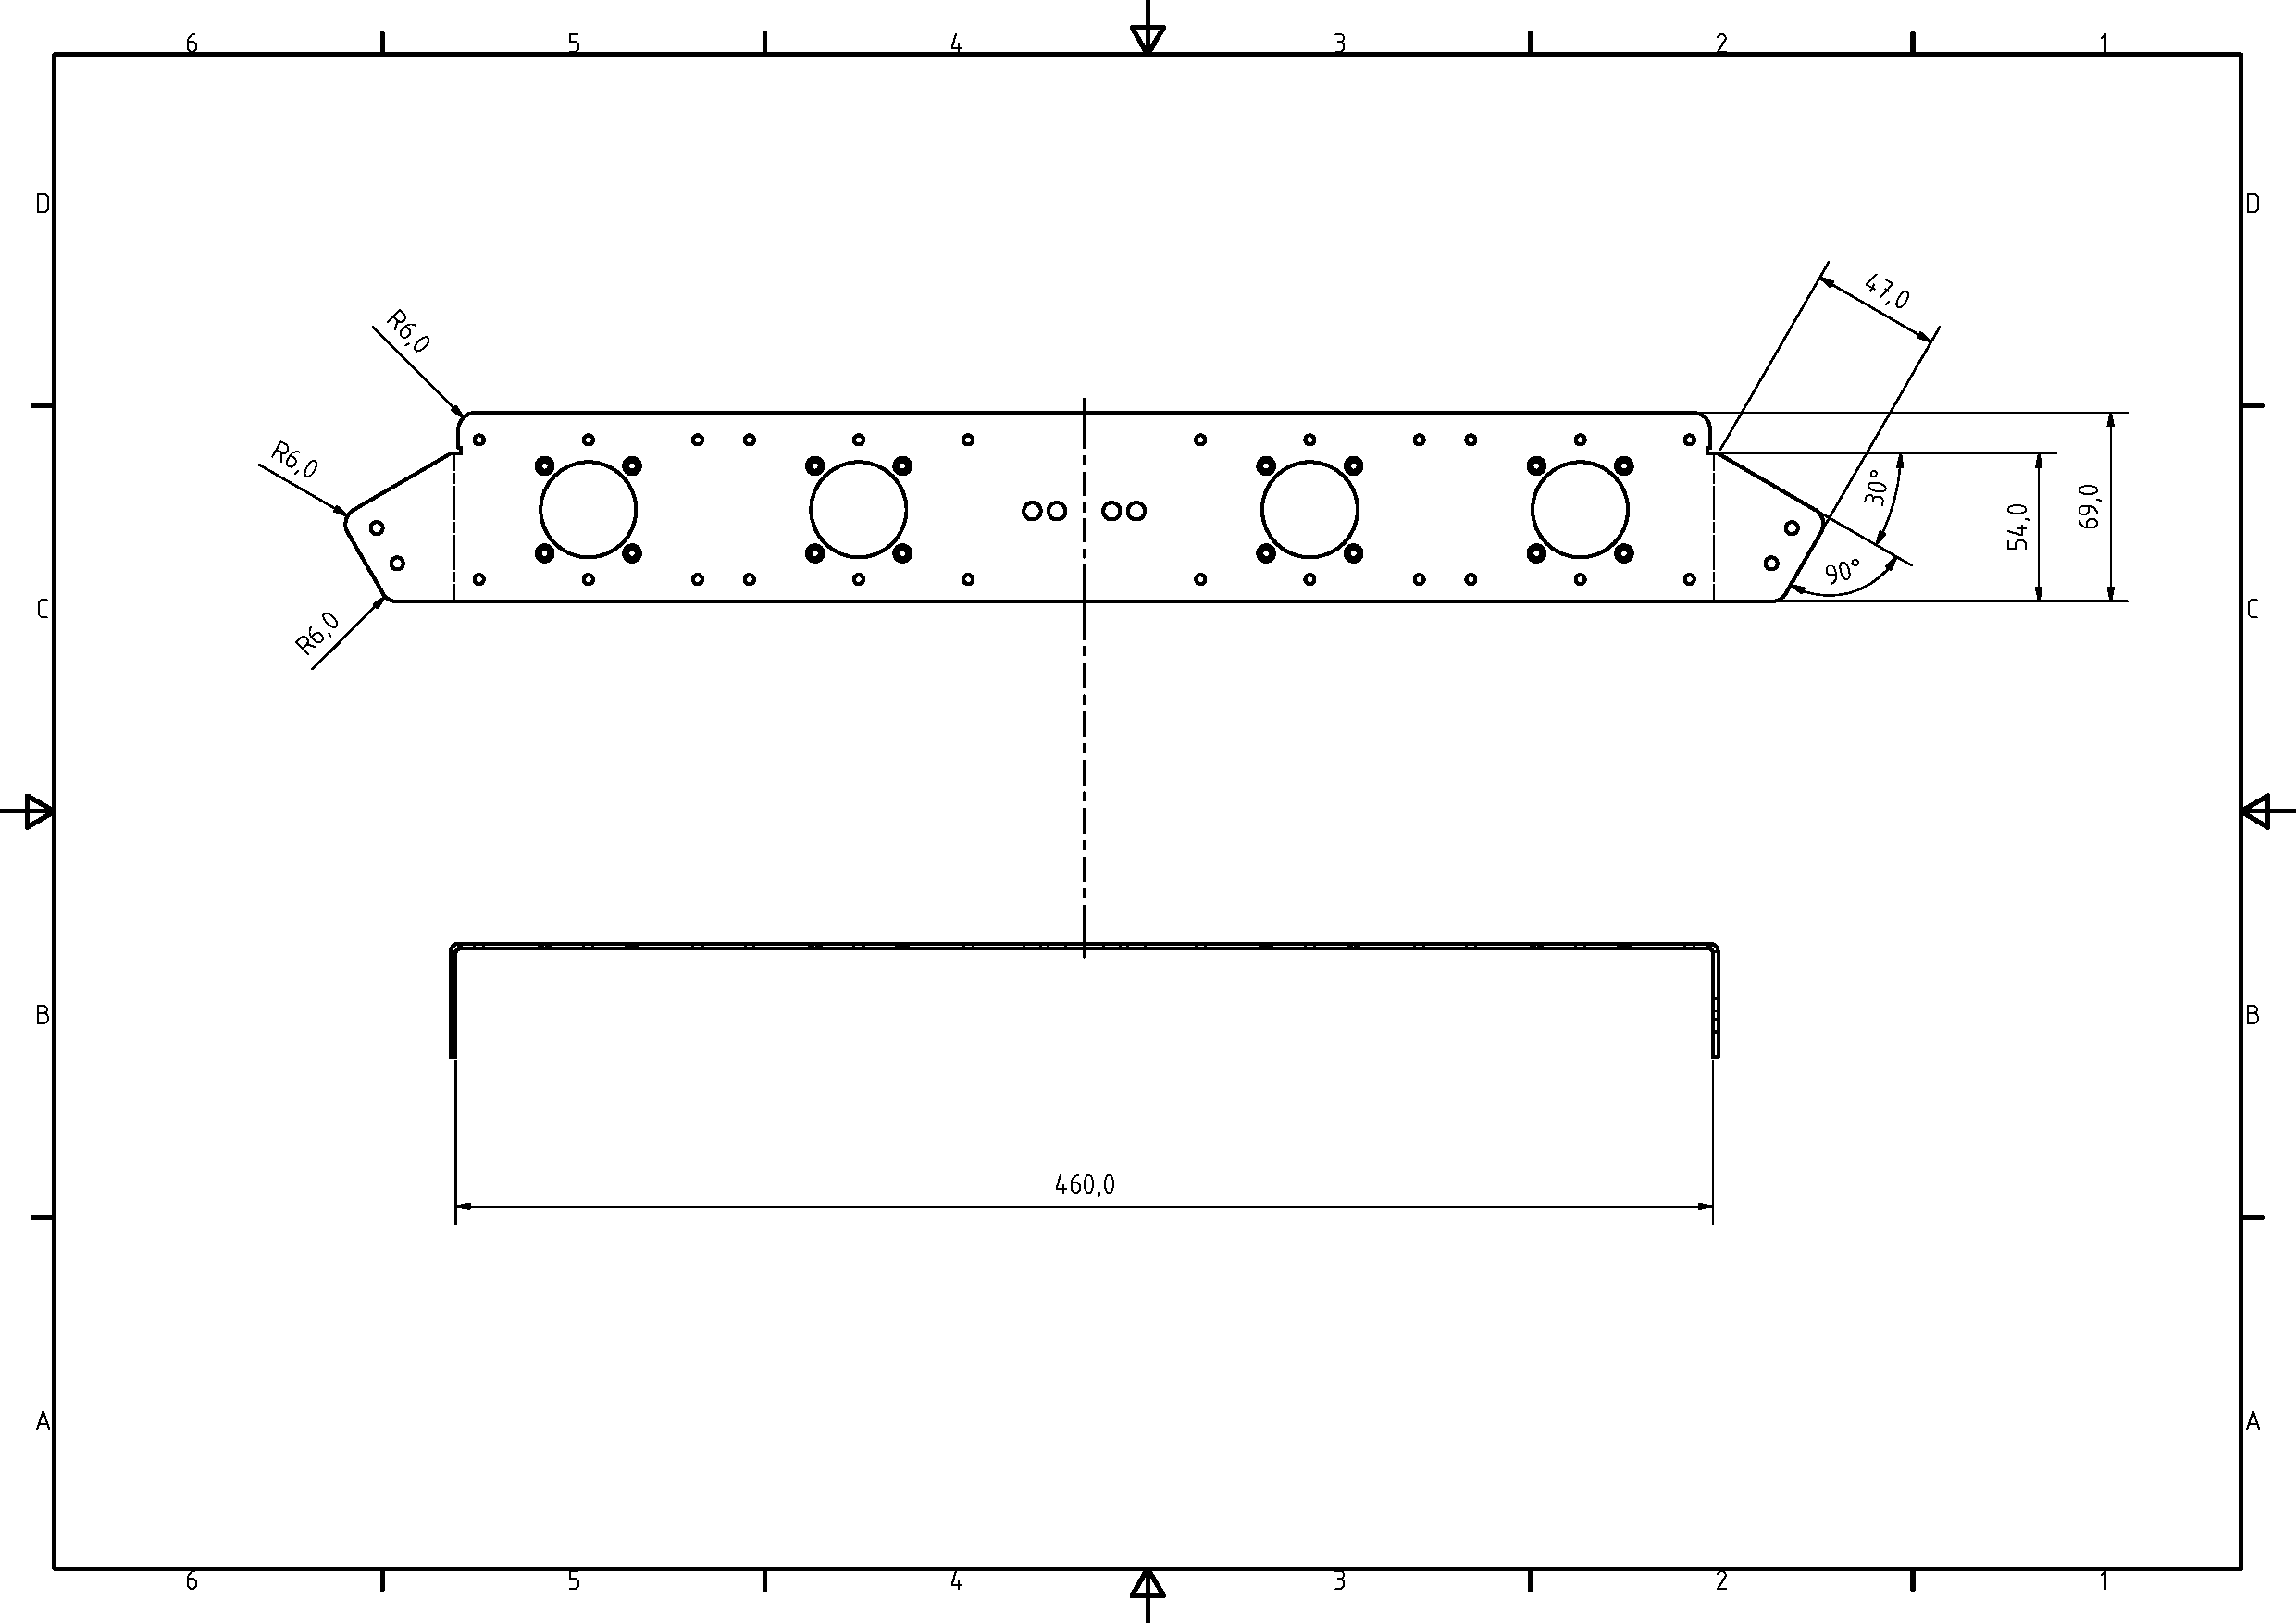
\includepdf[pages=-,fitpaper]{inc/drawing_v_mount.pdf}
